\begin{egBox}{Unit Circle -- Cutting and Glueing}[eg:18.1]
    Let us consider the following functions between the unit circle \( S \) and
    the half open interval (insert image).
    Assume both are equipped with their Euclidean topologies.

    \baseSkip

    \wrapBox{Cutting}

    \begin{figure}[H]
        \centering
        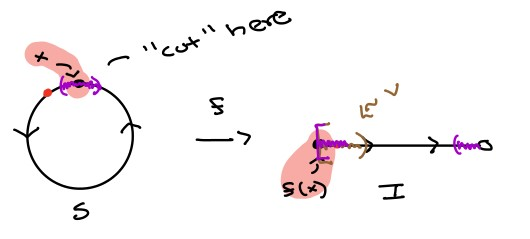
\includegraphics[ width = 0.4\linewidth ]{figures/Section 18/eg18-1-1.jpg}
        \caption{Open Neighborhoods of \( x \) after Cutting}
        \label{fig:18-1}
    \end{figure}

    Notice that an open neighborhood of \( x \) in \( S \) contains points that
    are left and right of \( x \), but an open neighborhood of \( x \) in the half-open interval consists of a smaller half-open interval.
    In Figure (\ref{fig:18-1}), the open neighborhood of \( x \) in \( S \) is 
    defined as \( U \), and the open neighborhood of \( x \) in the half open
    interval is defined as \( V \).
    If our function \( f \) is the action of cutting the unit circle at \( x \),
    then we can see in Figure (\ref{fig:18-1}) that the image of \( U \) under 
    this function is not contained in \( V \) -- there are values at the
    right-end of our half-open interval that are not contained in \( V \).

    
    \wrapBox{Cutting}

    \begin{figure}[H]
        \centering
        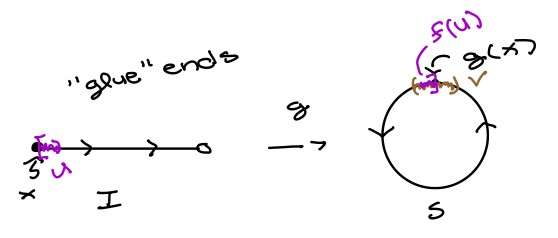
\includegraphics[ width = 0.4\linewidth ]{figures/Section 18/eg18-1-2.jpg}
        \caption{Open Neighborhoods of \( x \) after Glueing}
        \label{fig:18-2}
    \end{figure}

    In Figure (\ref{fig:18-2}), the open neighborhood of \( x \) in the 
    half-open interval is defined as \( U \), and the open neighborhood of 
    \( x \) in \( S \) is defined as \( V \).
    In this scenario, our function \( g \) is now defined to be the action 
    of glueing the half-open interval into a unit circle.
    We can see in Figure (\ref{fig:18-2}) that the image of \( U \) under 
    this function is contained in \( V \) this time around.
    Thus, \( g \) is continuous.

    \baseSkip

    In general, we have that "cutting" is something that is not continuous.
    However, "glueing" is continuous.
    This example also shows that for a continuous function, its inverse 
    need not be continuous as well.
\end{egBox}

\begin{egBox}{Projections are Continuous Functions}[eg:18.2]
    Let \( X = \prod_{ i \in I } X_{ i } \) be a product of topological spaces.
    We fix an index \( k \in I \) and consider: \( \mathrm{proj}_{ k }: X \rightarrow X_{ k } \). 
    These functions are always continuous, whether we equip \( X \) with the 
    product topology or the box topology.

    \baseSkip

    This can be easily proven by noting that the inverse image of an open 
    subset of \( X_{ k } \) under 
    \( \mathrm{proj}_{ k } \) is open in the product topology (and therefore
    also in the at least as fine box topology).
    I.e., we have that whenever \( V \subset X_{ k } \) is open in 
    \( X_{ k } \), \( \mathrm{proj}_{ k }^{ -1 } ( V ) \) is open in \( X \).
    Thus, \( \mathrm{proj}_{ k } \) is continuous.
\end{egBox}

\begin{egBox}{Continuity of a Function (Codomain given by a basis)}[eg:18.3]
    Let \( f: X \rightarrow Y \) be a function between topological spaces where the topology on \( Y \) is generated by a basis. 
    Assume \( f^{ -1 } ( B ) \) is open whenever \( B \) is a basic open subset 
    of \( Y \).
    We want to show that \( f \) is continuous.

    \baseSkip

    Let \( V \subset Y \) be open.
    Since \( Y \) is generated by a basis, we have that \( V = 
    \bigcup_{ i \in  I } B_{ i } \) where \( B_{ i } \) are some basic open subsets.
    Using the properties of inverse images, we see that 
    \begin{equation*}
        f^{ -1 } ( V )
        =
        f^{ -1 } \left( \bigcup _{ i \in I } B_{ i } \right)
        =
        \bigcup _{ i \in I } f^{ -1 } ( B_{ i } )
    \end{equation*}
    Since each \( f^{ -1 } ( B_{ i } ) \) is open by assumption, we see that 
    \( f^{ -1 } ( V ) \) is a union of open subsets, which is still open.
    Thus, \( f^{ -1 } ( V ) \) is open in \( X \).
\end{egBox}

\begin{egBox}{Continuity in the Discrete and Trivial Topology}[eg:18.4]
    Let \( f: X \rightarrow Y \) be a function between topological spaces.
    We want to show that 
    \begin{enumerate}[label = (\alph*)]
        \item \( f \) is automatically continuous if \( X \) has the discrete
            topology.
        \item \( f \) is automatically continuous if \( Y \) has the trivial 
            topology.
    \end{enumerate}

    \baseSkip

    \wrapBox{a}

    Let's say that we are given some \( V \) that is open in \( Y \).
    It follows that \( f^{ -1 } ( V ) \) must be some subset of \( X \), but 
    since we have that \( X \) has the discrete topology, all subsets of \( X \)
    are open.
    Hence, we see that \( f^{ -1 } ( V ) \) is open as well, meaning that 
    \( f \) is continuous.

    \baseSkip

    \wrapBox{b}

    Let's now say that \( Y \) has the trivial topology -- this means that 
    the only open sets are \( \emptyset \) and \( Y \) itself.
    It is clear to see that \( f^{ -1 } ( \emptyset ) = \emptyset \), which
    is always an open set in \( X \).
    We also see that \( f^{ -1 } ( Y ) = X \), which is also an open set in 
    \( X \).
    Hence, we see that \( f \) is continuous as well.
\end{egBox}

\begin{egBox}{Continuity From the Right}[eg:18.5]
    Consider the function \( f: \mathbb{R} \rightarrow \mathbb{R} \) defined by
    \begin{equation*}
        f ( x )
        =
        \begin{cases} 
            0 &\quad x < 0
            \\
            1 &\quad x \geq 0   
        \end{cases}
    \end{equation*}
    This is evidently discontinuous at \( x = 0 \) when \( \mathbb{R} \) is
    given the standard topology.
    However it is continuous at \( x = 0 \) as a function 
    \( f: \mathbb{R}_{ \ell } \rightarrow \mathbb{R} \).
    In other words, it is continuous when the domain is equipped with the lower-
    limit topology.
    Thus, we see that continuity from the right is the same as continuity when
    the domain is equipped with the lower-limit topology.
    
    \begin{figure}[H]
        \centering
        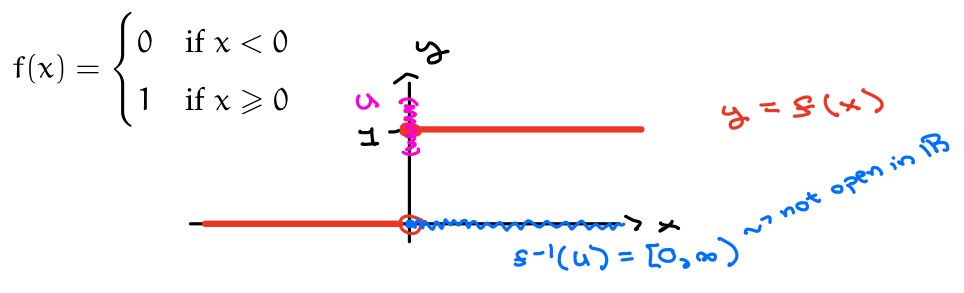
\includegraphics[ width = 0.5\linewidth ]{figures/Section 18/18-5-1.jpg}
        \caption{Continuity from the Right}
        \label{fig:18-4}
    \end{figure}
\end{egBox}

\begin{egBox}{A Non-example of a Homeomorphism}[eg:18.6]
    Glueing and Cutting are bijective, but we do not end up with a homeomorphism
    The issue is that glueing is continuous, but cutting is not.
\end{egBox}